
\cleardoublepage


\chapter{Experimental Validation}




\section{Spectral Unfolding}

\subsection{Methods and Parameters}

% the responses and response functions were used with the unfolding methods described in ch2 to obtain solution spectra
% the bss and ft_au results were first considered separately, then combined
% both the gravel and maxed unfolding algorithms were used with these data
% for gravel, 50 iterations were used
% for maxed, the parameter omega was set using the number of detectors for each dataset, 9 for the foil tube, 7 for the bss, and 16 for the combined set
% then, the maxed portion was repeated, while first scaling the default spectrum

\subsection{Results and Discussion}

% the figures below show the results from the three unfoldings

\begin{figure}[htb]
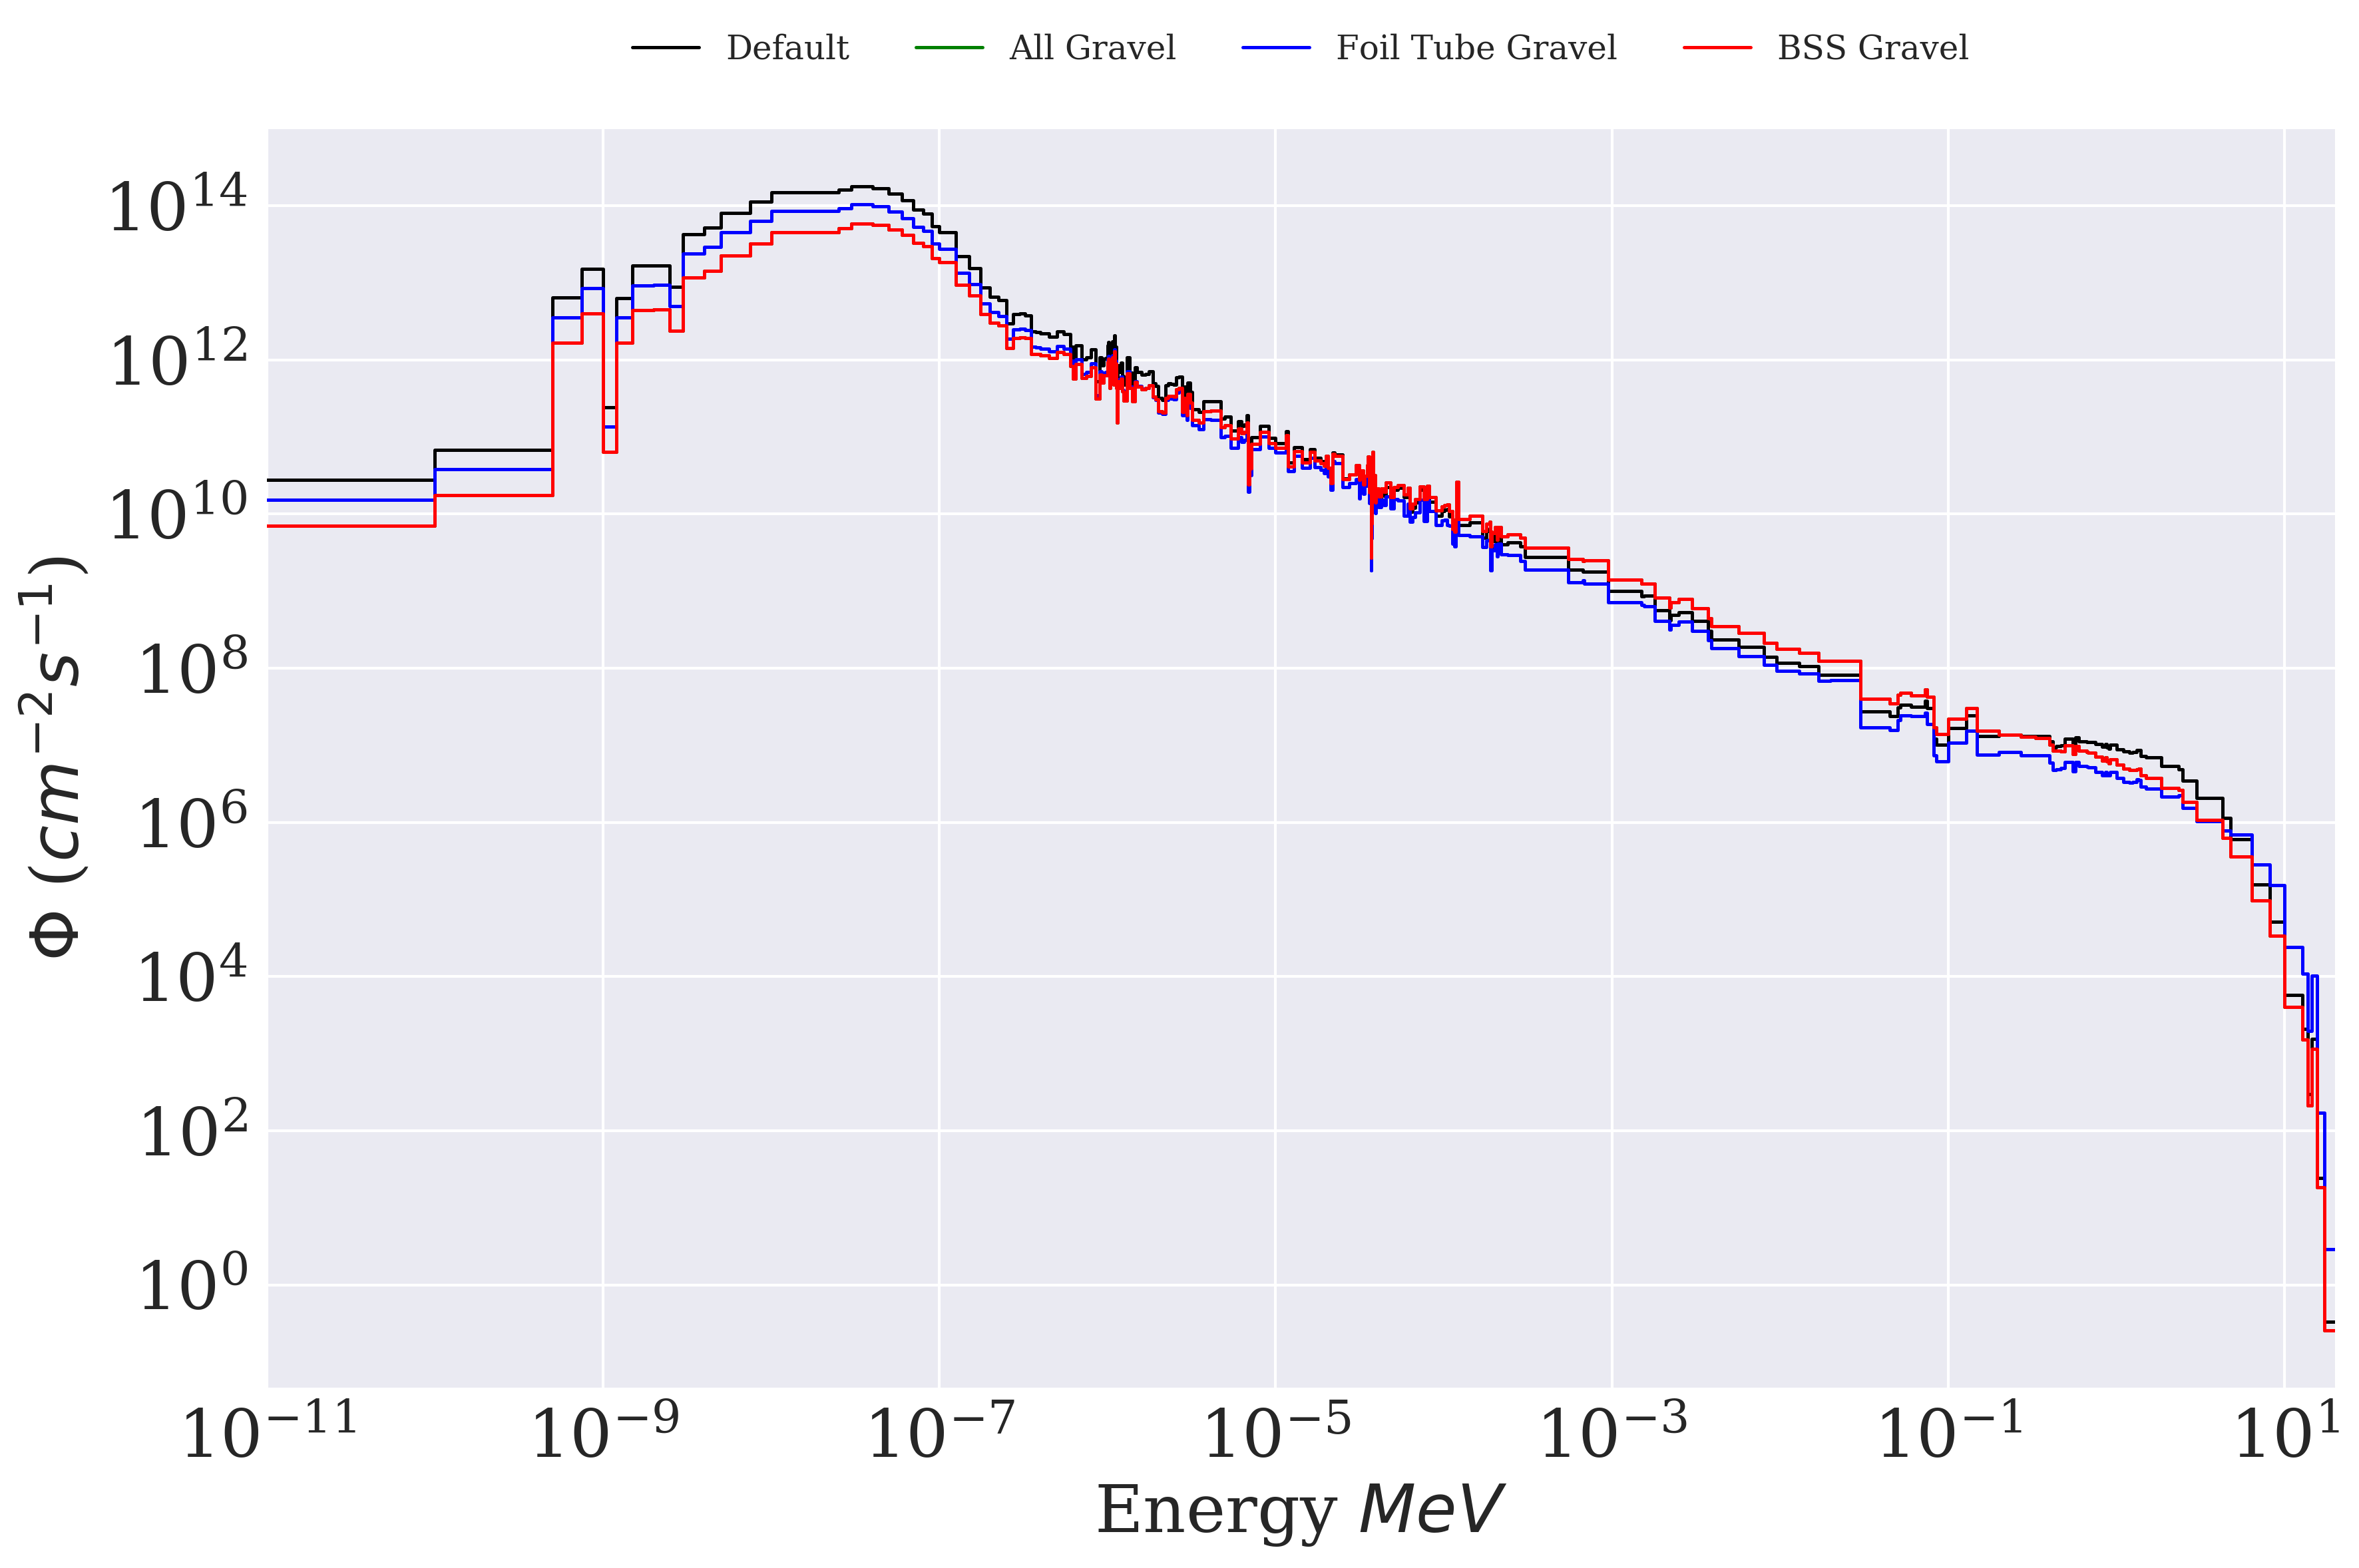
\includegraphics[height=4in]{tex/figures/unfolded_gr.png}
\caption[]{}
\label{fig:unfolded_gr}
\end{figure}

% here gravel results are presented first
% as seen in the figure, the bss and ft_au results show good agreeance with one another
% all of the major features from the default spectrum are preserved
% the ft_au results unfold to a slightly higher thermal flux than the bss where as the bss show slightly higher fast region
% the combined results cannot be seen as they are covered by the ft_au
% this is because with gravel, smaller error responses are weighted heavier and the errors are much smaller for the gold foils than for the bss

\begin{figure}[htb]
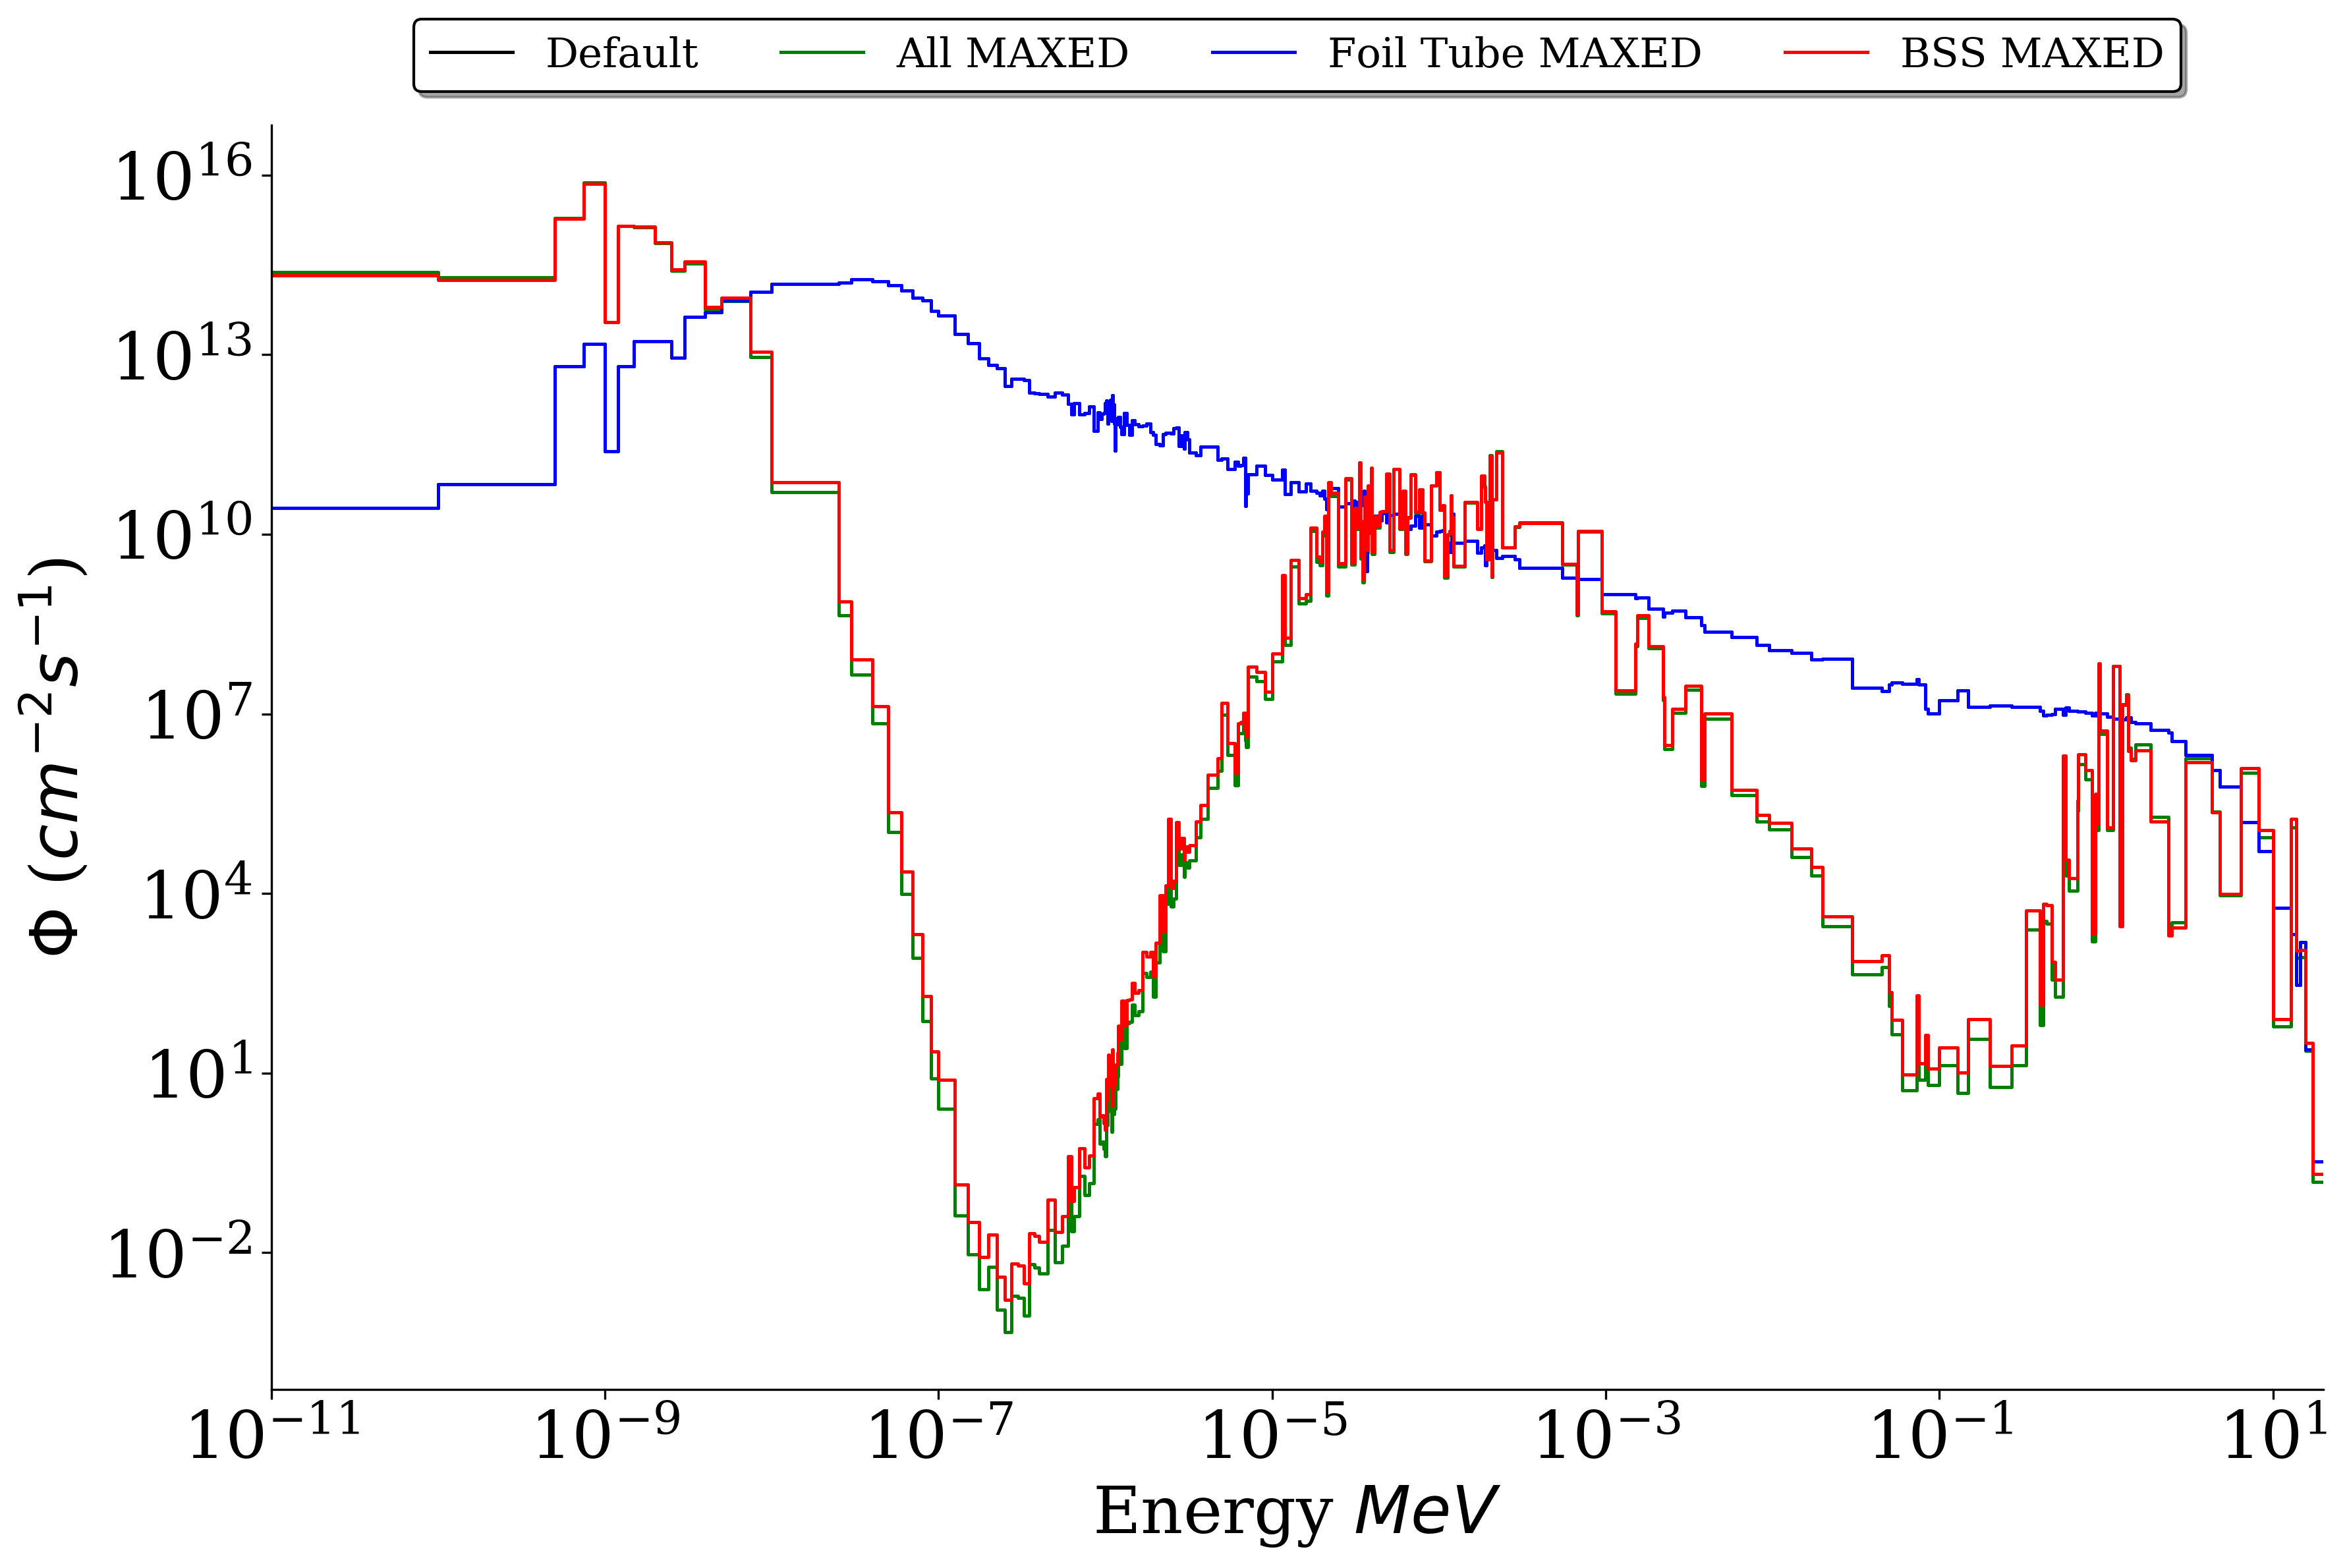
\includegraphics[height=4in]{tex/figures/unfolded_mx.png}
\caption[]{}
\label{fig:unfolded_mx}
\end{figure}

% these results shown in FIG are from the maxed unfolding.
% in the case of the bss and combined case, the results produced are very unphysical
% this is likely due to the fact that the spectrum is trying to fit the data while staying close to the default spectrum
% in the ft_au case, the default spectrum remains unchanged, indicating that the default spectrum actually represents a decent fit of the data

\begin{figure}[htb]
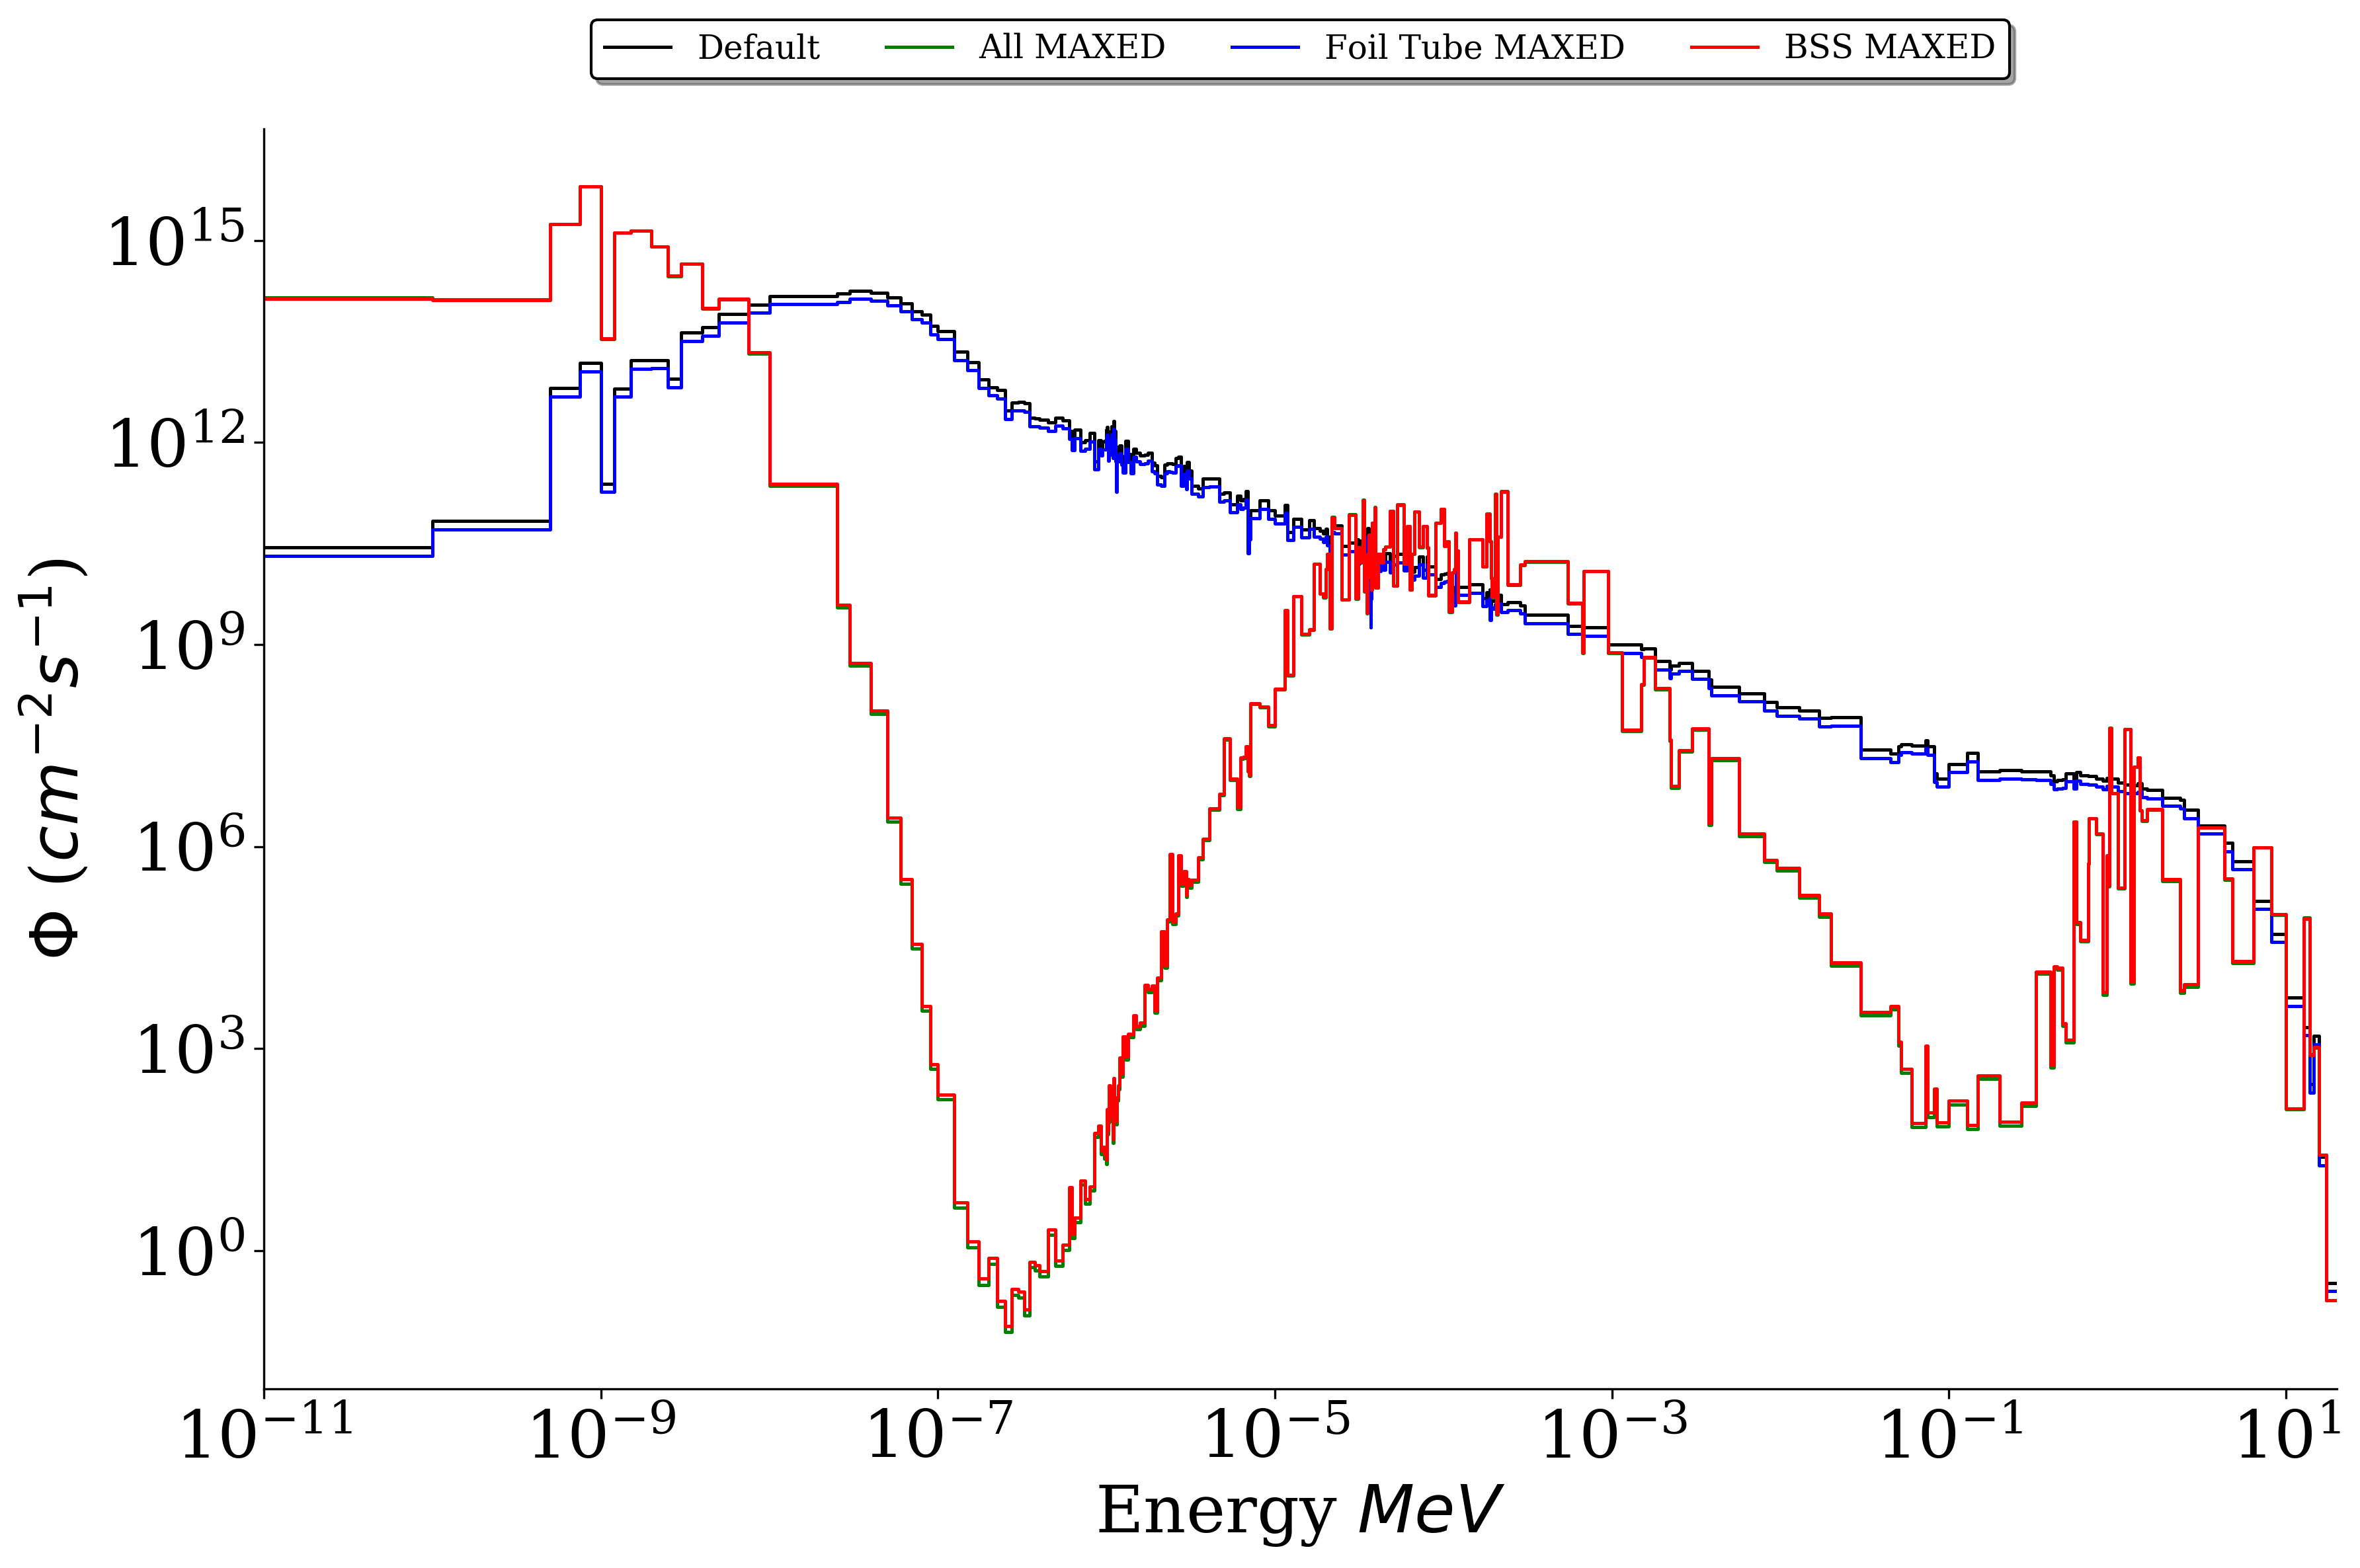
\includegraphics[height=4in]{tex/figures/unfolded_mx_sc.png}
\caption[]{}
\label{fig:unfolded_mx_sc}
\end{figure}

% although it was hypothesized that scaling the spectrum would results in a less erratic answer, the results here are very similar in characteristics to the unscaled maxed results
% the bss and combined cases are still unphysical, and the ft_au remaines unperturbed


